\section{Kalibrierung}
Um die Energiemessung des Detektors zu kalibrieren, werden zwei bekannte Elemente als Target benutzt. Die gemessenen Kanten der Spektren können dann dazu genutzt werden, mit dem für die Elemente bekannten K-Faktor eine lineare Kanal-Energie-Kalibrierung durchzuführen. 

Die Elemente werden so ausgewählt, dass die K-Faktoren möglichst unterschiedlich sind, damit die Steigung der Kalibrierungsfunktion über einen möglichst großen Bereich berechnet wird. Einen besonders kleine K-Faktor hat Kohlenstoff und einen großen K-Faktor hat Gold.

Wie auch im eigentlichen Versuch sind die Kanten verschmiert und es wird daher eine Methode benötigt, den mittleren Wert der Kante zu finden. Auf dem PC werden dazu im Analyseprogramm ein maximaler Wert der Kante $A$ und eine Wert unterhalb der Kante $B$, bei dem keine Rückstreuung mehr vorhanden ist, ausgewählt. Mit dem Mittelwert $(A+B)/2$ sucht man dann den Kanal, der diesem Wert am nächsten kommt und nimmt diesen für die Kante an.

In den Abbildungen \ref{Kohlenstoff} und \ref{Goldprobe} finden sich die beiden aufgenommenen Spektren für Gold und Kohlenstoff. Auffällig im Spektrum für Gold ist die zweite, sehr viel kleinere Kante bei ca. 500keV neben der eigentlichen Au-Kante bei ca. 1850keV. Diese entspricht dem unter der dünnen Goldschicht vorhandenen Kohlenstoffkern, wodurch die Kohlenstoffkante also hier in beiden Spektren erkennbar ist. 

\begin{figure}[htbp]  
     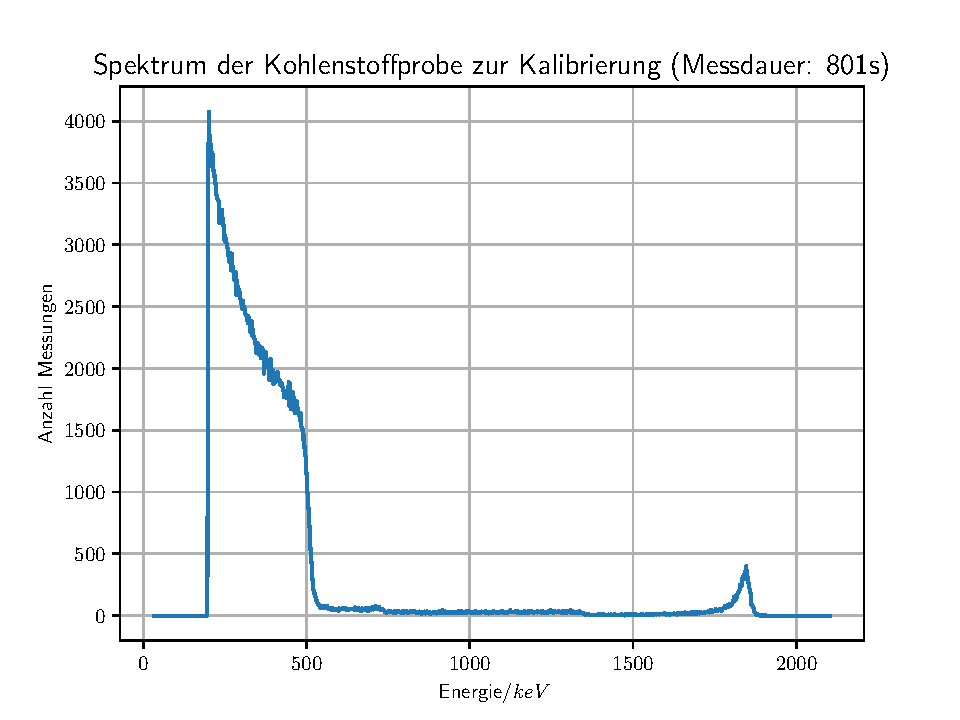
\includegraphics{Kohlenstoffprobe_zur_Kalibrierung.pdf}
  \caption{Kohlenstoffprobe zur Kalibrierung}
  \label{Kohlenstoff}
\end{figure}

\begin{figure}[htbp]  
     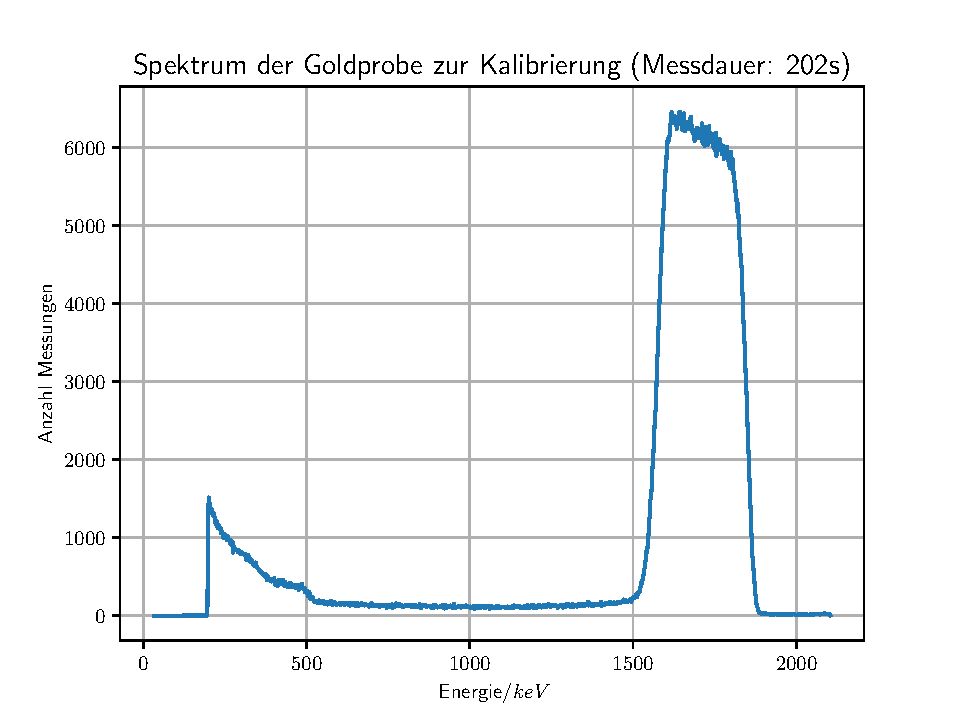
\includegraphics{Goldprobe_zur_Kalibrierung.pdf}
  \caption{Goldprobe zur Kalibrierung}
  \label{Goldprobe}
\end{figure}

Aus den Spektren wurden für Kohlenstoff und Gold bei einer Strahlenergie $2000keV$ folgende Werte gefunden:\\\\
\begin{tabular}{|l|l|l|l|l|}
\hline
 & K-Faktor & Energie/keV & Kanal\\
 \hline
 C & $0,252$ & $504$ & 234\\
 \hline
 Au & $0,9223$ & $1844,6$ & 896\\
 \hline
\end{tabular}\\\\
Die lineare Kalibrierungsfunktion
\begin{equation}
 E(k)= a\cdot k + b
\end{equation}
wird bestimmt, indem zuerst die Steigung $a$ berechnet wird:
\begin{equation}
 a = \frac{(1844,6 - 504)keV}{(896 - 234)Kanal}=2,025\frac{keV}{Kanal}
\end{equation}
Zuletzt wird $b$ bestimmt mit der Formel:
\begin{equation}
 b = 504keV - 2,025 keV\cdot 234 = 30,13 keV
\end{equation}

Mit der Formel
\begin{equation}
 E(k)=2,025\frac{keV}{Kanal}\cdot k + 30,13keV 
\end{equation}
werden ab hier alle gemessenen Energien der zurückgestreuten Helium-Ionen gemessen.
